\documentclass{beamer}

\newcommand{\set}[1]{\left\{ #1 \right\}}
\newcommand{\abs}[1]{\left\lvert #1 \right\rvert}

\newcommand{\N}{\mathbb{N}}
\newcommand{\Z}{\mathbb{Z}}
\newcommand{\R}{\mathbb{R}}
\newcommand{\F}{\mathbb{F}}
\renewcommand{\S}{\mathfrak{S}}

\newcommand{\Top}{\mathsf{Top}}
\newcommand{\Grp}{\mathsf{Grp}}
\newcommand{\Ab}{\mathsf{Ab}}
\newcommand{\Simp}{\mathsf{Simp}}
\newcommand{\Ch}{\mathsf{Ch}}


\makeatletter
\newcommand*{\defeq}{\mathrel{\rlap{%
    \raisebox{0.3ex}{$\m@th\cdot$}}%
  \raisebox{-0.3ex}{$\m@th\cdot$}}%
	=
}
\makeatother

\DeclareMathOperator{\im}{im}

% Category theory
\newcommand{\longto}{\longrightarrow}
\newcommand{\into}{\hookrightarrow}

\newcommand{\MKNN}{M\( k \)NN }
\newcommand{\hombound}[2]{\bar{\partial}_{#1}^{#2}}
\newcommand{\hbound}[1]{\bar{\partial}^{#1}}

% Cycles and boundaries
\newcommand{\cyc}[1]{\ker{\partial}_{#1}}
\newcommand{\bound}[1]{\im{\partial}_{#1}}

\newcommand{\pcyc}[2]{\ker{\partial}_{#1}^{#2}}
\newcommand{\pbound}[2]{\im{\partial}_{#1}^{#2}}


\usepackage[english]{babel}
\usepackage[utf8]{inputenc}
\usepackage[T1]{fontenc}
\usepackage{lmodern}

\usepackage{graphicx}
\graphicspath{{figs/}{../figs/}}

\usepackage{amsmath, amssymb, mathtools}

\hypersetup{
	colorlinks,
	linkcolor = {red!50!blue},
	citecolor = {red!50!blue},
	urlcolor = {red!50!blue},
	linktoc = page
}

\title{}
\author{Arnau Mas}
\date{September 3rd 2020}


\begin{document}
\frame{\titlepage}

\section{The problem}

\begin{frame}
	\frametitle{What is radiomics?}
	\begin{itemize}
		\item Has its origins in the field of oncology: tumour imaging \pause
		\item Extract many \alert{radiomic features} from scans \pause
		\item Look for correlations between radiomic features and treatment response
	\end{itemize}
\end{frame}

\begin{frame}
	\frametitle{What is radiomics?}
	\begin{columns}
		\begin{column}{0.5\textwidth}
			\begin{block}{Benefits}
				\begin{itemize}
					\item Non-invasive
					\item More systematic
					\item Quantitative
				\end{itemize} \pause
			\end{block}		
		\end{column}
		
		\begin{column}{0.5\textwidth}
			\begin{block}{Drawbacks}
				\begin{itemize}
					\item May be hard to reproduce
					\item High dimensional feature spaces
					\item Limited number of cases
				\end{itemize} 
			\end{block}				
		\end{column}
	\end{columns}
\end{frame}

\begin{frame}
	\frametitle{TOPiomics}

	\begin{center}
		
\includegraphics[width = 3cm]{beamer/logo-cvc}
		\hfill
		
\includegraphics[width = 3cm]{beamer/logo-vhio}
	\end{center}

	\begin{itemize}
		\item TOPiomics is an ongoing collaboration between the Computer Vision Center (CVC) and the
			Vall d'Hebron Institute of Oncology (VHIO). \pause

		\item Main aim: early detection of patients with strange radiomic signatures,
			\emph{outliers}, for whom standard treatments could fail. \pause

		\item	Use \emph{topological data analysis}, hence TOPiomics (topological radiomics).

	\end{itemize}
\end{frame}

\begin{frame}
	\frametitle{Prior work}
	\begin{itemize}
		\item Progress thus far: use the \emph{mutual \( k \)-nearest neighbours} (\MKNN) graph to
			detect outliers. \pause
		\item Problem: there is a parameter that has to be fixed. It has to do with the scale
			at which we look at the data. \pause
		\item Idea: look at \emph{every} parameter value. \pause 
	\end{itemize}
	\centering \alert{This is persistence} 
\end{frame}

\section{An overview of homology}
\begin{frame}
	\frametitle{The elevator pitch}
	Algebraic topology studies topological spaces by computing algebraic invariants, namely
	with functors
	\begin{gather*}
		\Top \to \Grp \\ 
		\Top \to \Ab \\
		\Top \to \Ring \\
		\Top \to \Vect_K \\
				 \vdots
	\end{gather*}
	\pause
	Homology groups are one of these functors,
	\begin{equation*}
		H_n \colon \Top \to \Ab. 
	\end{equation*}
	\pause
	They come in many flavours, the simplest one is \emph{simplicial homology}, which works
	for \emph{simplicial complexes}. 
\end{frame}

\begin{frame}
	\frametitle{The ingredients of homology}
	\begin{columns}
		\begin{column}{0.5\textwidth}
			\begin{itemize}
				\item<1-> \emph{Simplex}. The convex hull of \alt<3->{an (ordered)}{a} set of
					\only<2->{(geometrically independent)} points. 
				\item<4-> \emph{Simplicial complex}, \( K \). Topological space assembled out of
					simplices glued along their faces. 
				\item<5-> \emph{Chain groups}, \( C_n(K) \). Free abelian groups generated by the \( n
					\)-simplices of a complex. 
			\end{itemize}		
		\end{column}

		\begin{column}{0.5\textwidth}
			\begin{center}
				\only<1-3>{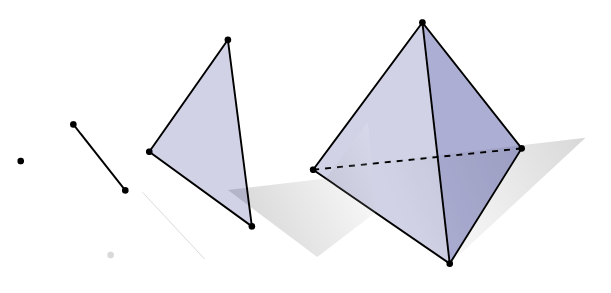
\includegraphics[scale=0.3]{beamer/simplices}}	
				\includegraphics<4->[scale=0.1]{beamer/complex}	
			\end{center}
		\end{column}
	\end{columns}
	
	\uncover<5>{
		\begin{block}{Remark}
			In the combinatorial picture, the geometrical requirements are dropped and one speaks
			of \emph{abstract} simplices, \emph{abstract} simplicial complexes, etc.
		\end{block}
	}
\end{frame}

\begin{frame}
	\frametitle{The boundary morphism}
	\begin{block}{Orientation}
		The simplex generated by \( p_0, \dots, p_n \) is written \( [p_0, \dots, p_n] \). The
		ordering determines an orientation, and we require that flipping orientation implies a
		change of sign in \( C_n(K) \), e.g.
		\begin{equation*}
			[p_0, p_1, \dots, p_n] = -[p_1, p_0, \dots, p_n]. 
		\end{equation*}
		\pause
		The chain groups are not really free!
	\end{block}
\end{frame}

\begin{frame}
	\frametitle{The boundary morphisms}
	Define the boundary morphism \( \partial_n \colon C_n(K) \to C_{n-1}(K) \) by
	\begin{equation*}
		\partial_n [p_0, \dots, p_n] \defeq \sum_{k = 0}^{n} (-1)^k [p_0, \dots, \hat p_k,
		\dots, p_n]
	\end{equation*}
	\pause
	\centering 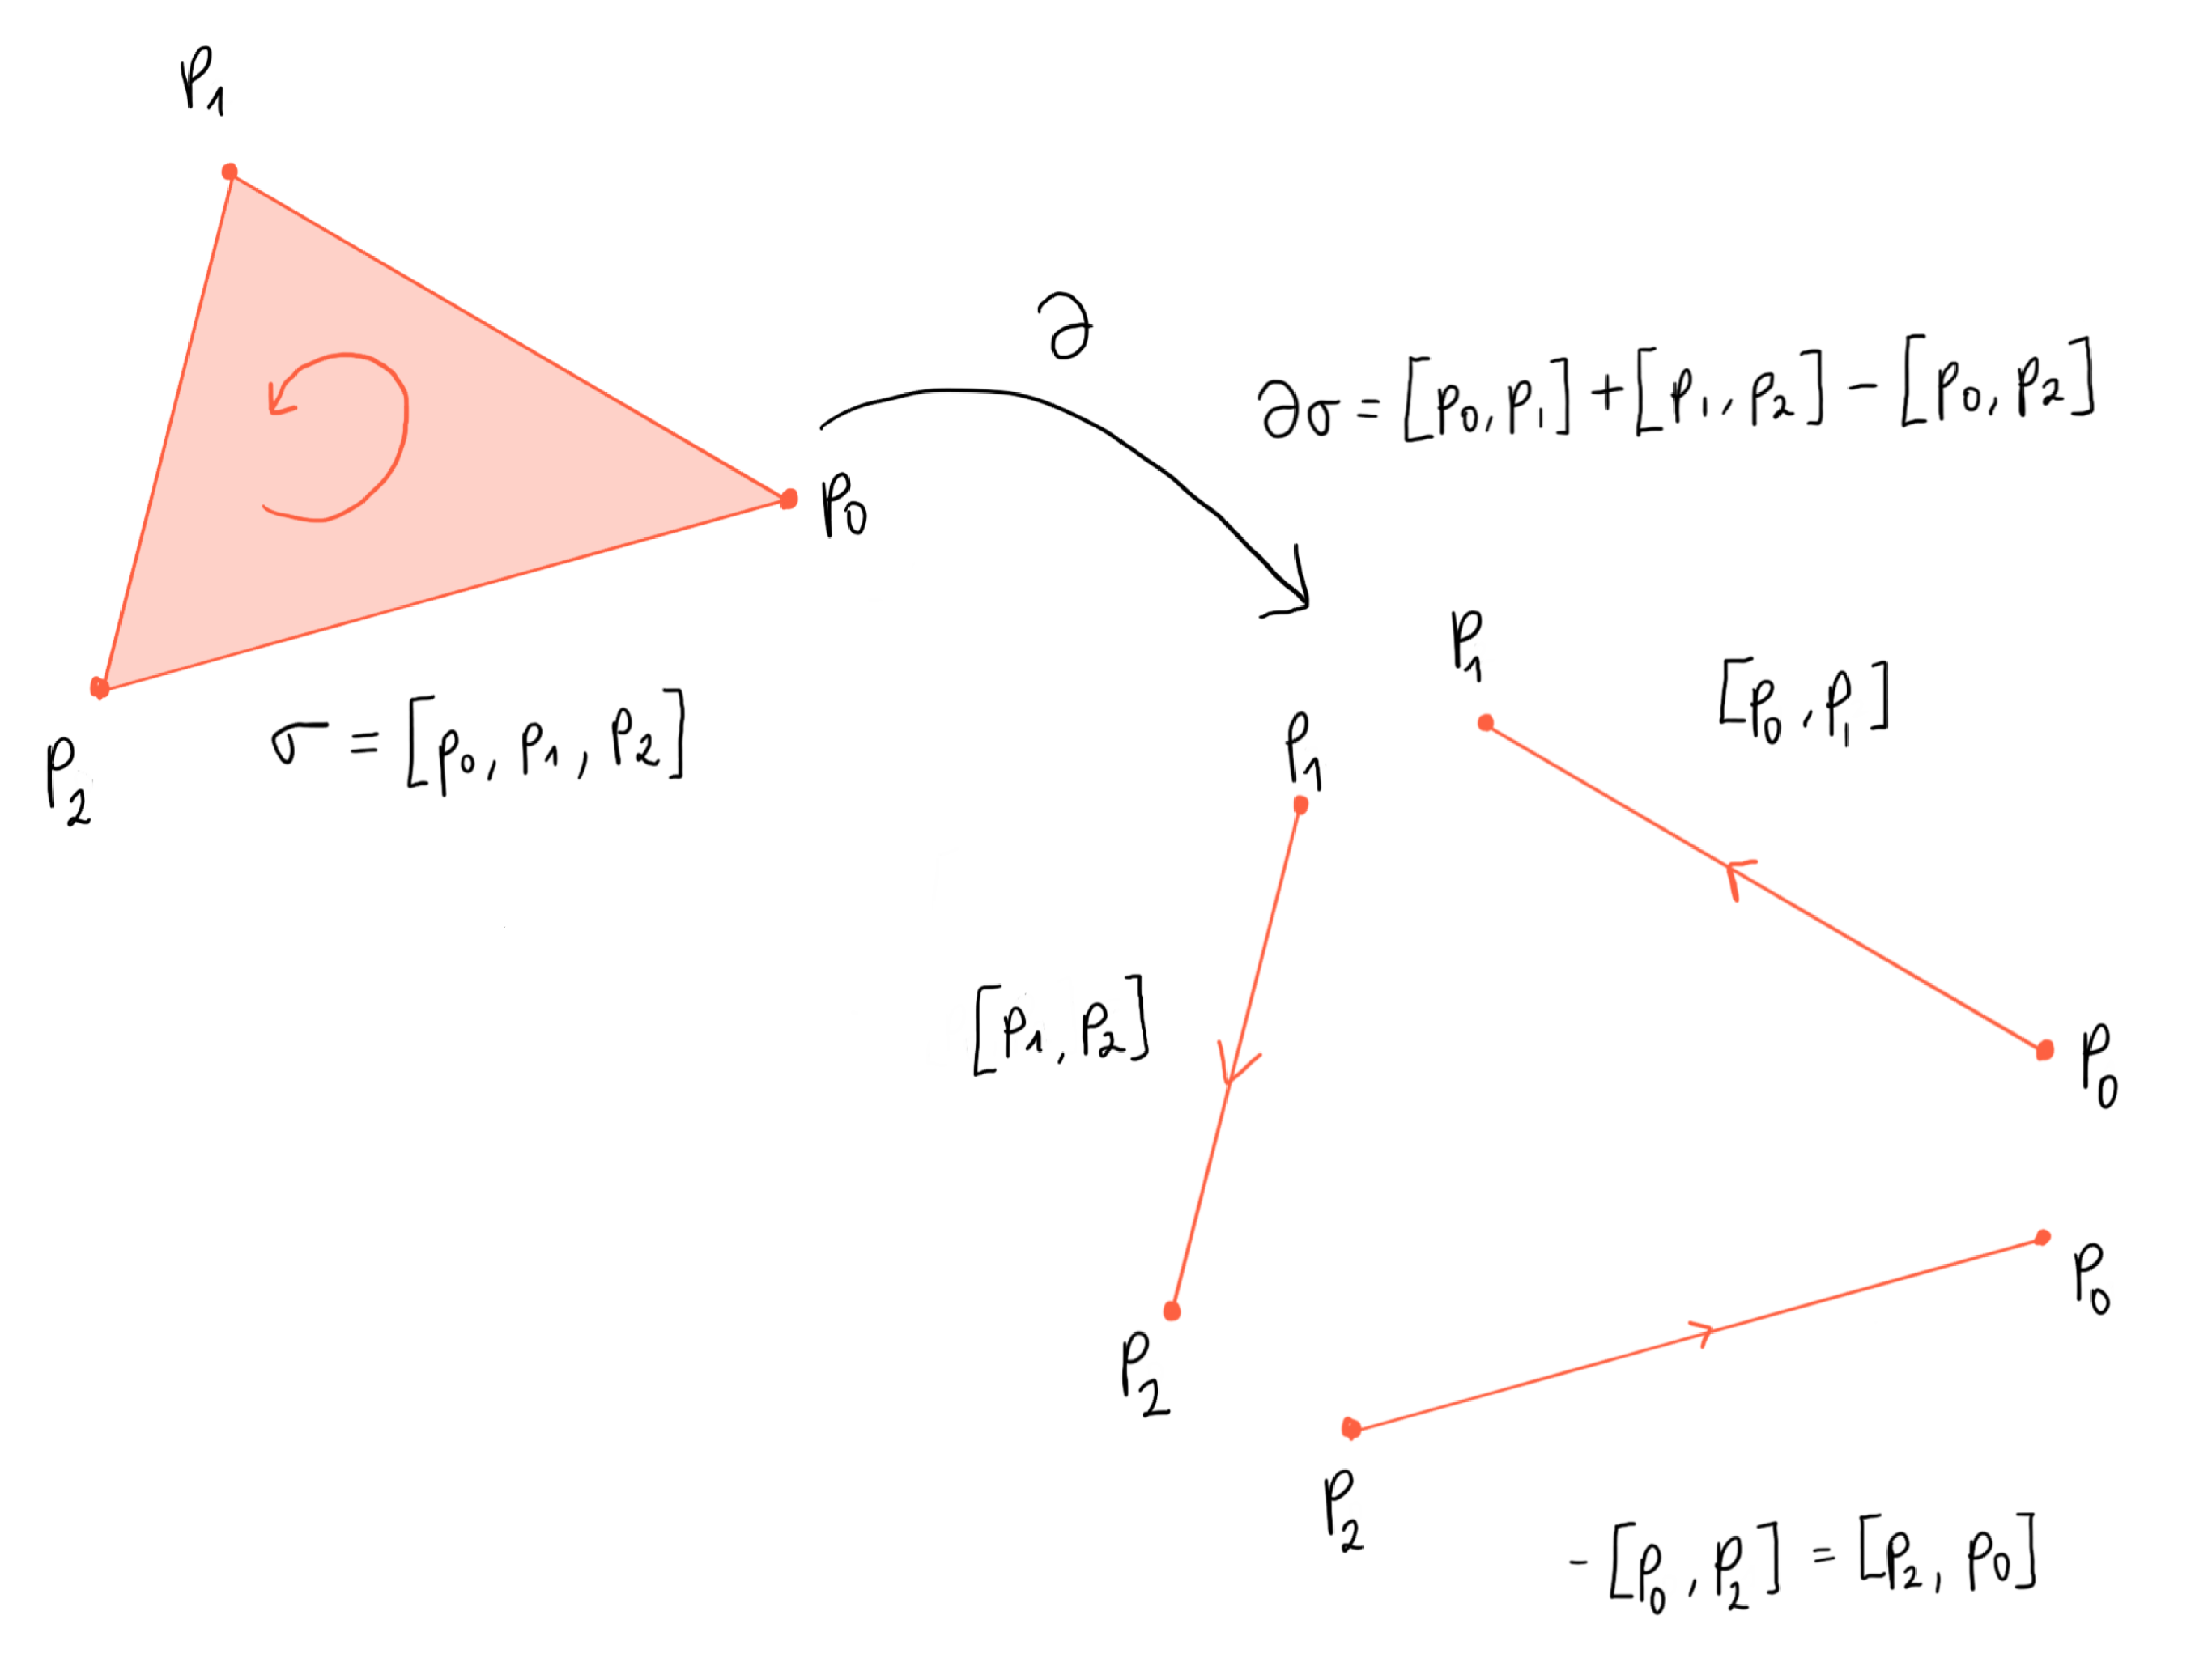
\includegraphics[width=0.7\textwidth]{drawings/boundary}
	
\end{frame}	

\section{The detector}


\section{The results}
\begin{frame}
	\frametitle{A run with toy data}
	\centering
	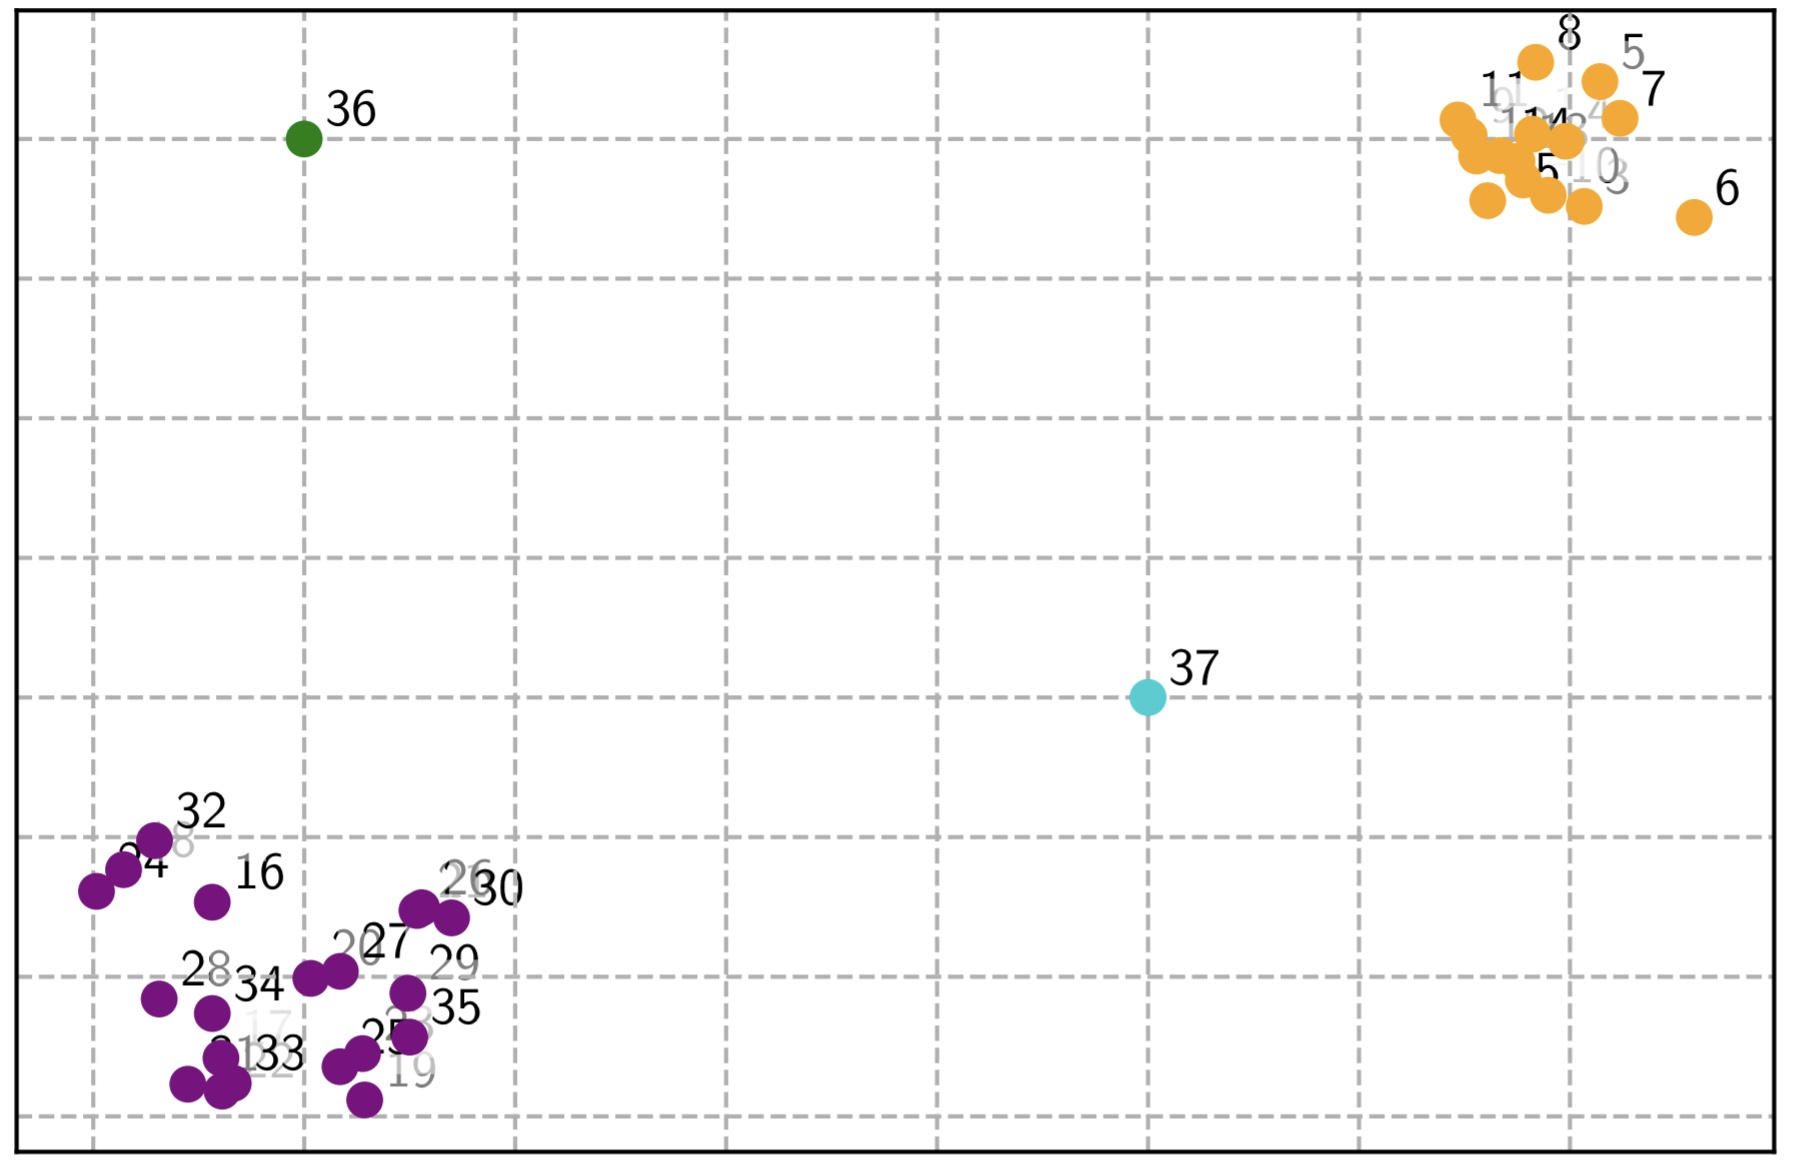
\includegraphics[width=\textwidth]{beamer/clusters}
\end{frame}

\begin{frame}
	\frametitle{A run with toy data}
	\centering
	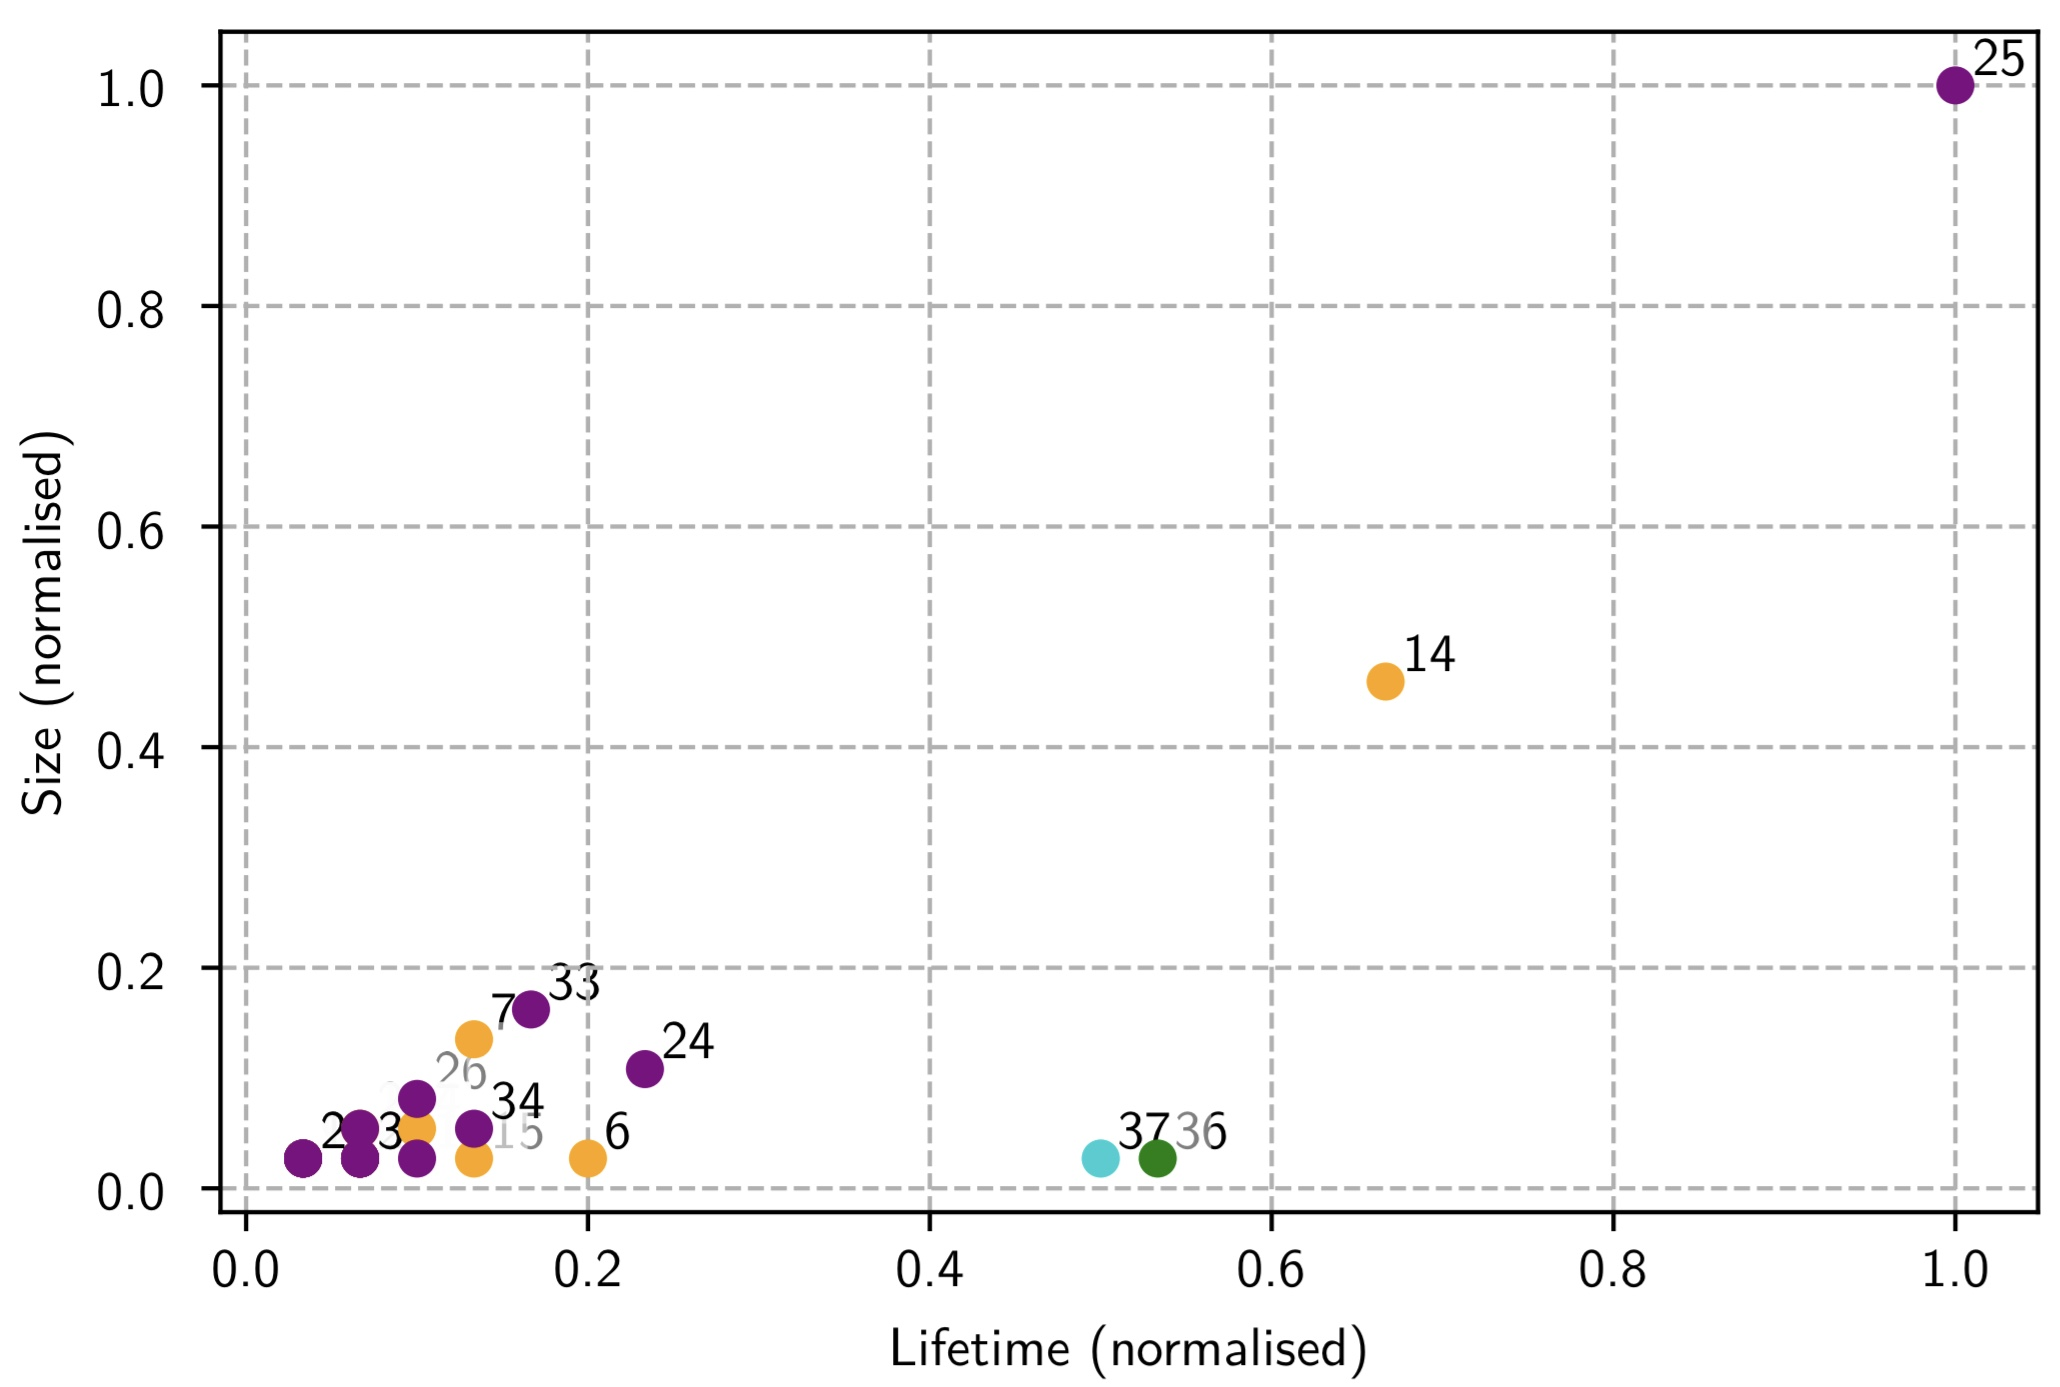
\includegraphics[width=\textwidth]{beamer/toy-results}
\end{frame}

\end{document}
